\section{Computational Results}
\label{sec:results}
In this section we consider an example from
\cite{cesinh}. The formulation of the transport
problem is taken from \cite{ctk:jeff1}. The equation for the angular
flux \(\psi\) is

\begeq
\label{eq:transportgs}
\mu \frac{\partial \psi}{\partial x} (x,\mu) + \Sigma_t(x) \psi(x,\mu) =
\frac{1}{2} \left[ \Sigma_s(x) \int_{-1}^1 \psi(x, \mu') \dmup + q(x) \right]
 \mbox{ for } 0 \le x \le \tau
\endeq

The boundary conditions are

\[
\psi(0, \mu) = \psi_l(\mu), \mu > 0; \psi(\tau, \mu) = \psi_r(\mu),
\mu < 0.
\]

In the computaions we use
\[
\tau=5, \Sigma_s(x) =\omega_0 e^{-x/s},  \Sigma_t(x) = 1, q(x) = 0, \psi_l(\mu) = 1, \psi_r(\mu) = 0,
\]
and consider two cases $s=1$ and $s=\infty$ 

\subsection{Using Krylov Linear Solvers}
\label{subsec:krylov}

We use two krylov methods \cite{ctk:roots}, GMRES \cite{gmres} and
Bi-CGSTAB \cite{bicgstab}.

The linear and nonlinear solvers come from the Julia package
\href{https://github.com/ctkelley/SIAMFANLEquations.jl}{SIAMFANLEQ.jl}
\cite{ctk:siamfanl}. The documentation for these codes is in the
\href{https://github.com/ctkelley/NotebookSIAMFANL}{Juila notebooks}
\cite{ctk:notebooknl} and the book \cite{ctk:fajulia}
that accompany the package. 

\subsection{Source Iteration and Krylov Methods}


\subsection{QMC and Krylov Linear Solvers}
\label{qmc-and-krylov-linear-solvers}

I can solve the QMC linear problem with both Krylov methods now and,
just like the classical case, I'm seeing fewer than half of the number
of transport sweeps. Herewith the results for N=1000 and Nx= 100.

\begin{figure}[t]%[!htbp]
  \centering
  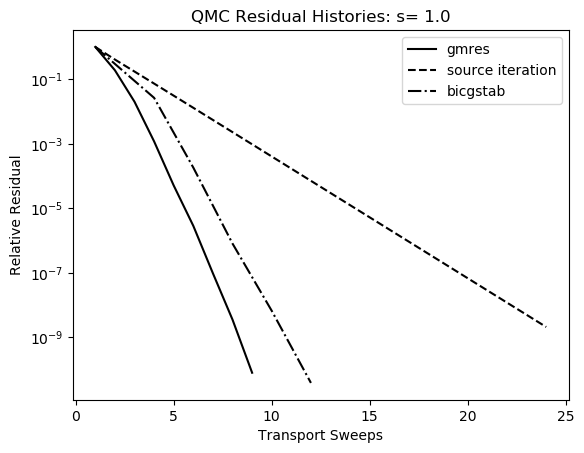
\includegraphics[trim = 10mm 0mm 15mm 15mm, width=70mm]{FIGURES/seqone.png}
  \caption{$s = 1$}
  \label{fig:easy}
\end{figure}

\begin{figure}[t]%[!htbp]
  \centering
  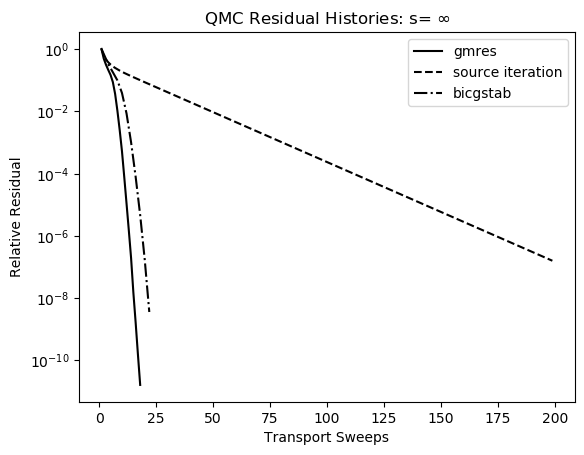
\includegraphics[trim = 10mm 0mm 15mm 15mm, width=70mm]{FIGURES/seqinf.png}
  \caption{$s = \infty$}
  \label{fig:hard}
\end{figure}

\subsection{Validation and calibration study}
\label{validation-and-calibration-study}

We conclude this section with a validation study. We compare the
QMC results with the results from \cite{cesinh}. The results
in \cite{cesinh} are exit distributions and are accurate to 
six figures. We have duplicated those results with an $Sn$ computation
on a fine angular and spatial mesh.

{\bf Sam, Ryan, should we use more or different values of $N$ and $Nx$?}

For $N = 1000$ and $Nx=100$ we obtain the cell-average fluxes from
the QMC approximation. We then use a single Sn transport sweep to recover
the exit distributions from the QMC cell-average fluxes. We report
the results and the corresponding results from \cite{cesinh} in 
Tables~\ref{tab:cesone} and \ref{tab:cesinf}.

The exit distributions, as is clear from Table~\ref{tab:cesone}
can vary by five orders of magnitude. Even so, the results from QMC
agree with the benchmarks to roughly two figues.

\begin{table}
\centering
\caption{Exit Distributiions: $s = 1$}
\label{tab:cesone}
\centerline{
\begin{tabular}{lllll}
 & \multicolumn{2}{c}{Garcia/Siewert}
 & \multicolumn{2}{c}{QMC}\\
\hline
    $\mu$ &$\psi(0, -\mu)$ &$\psi(\tau, -\mu)$ &$\psi(0, -\mu)$ &$\psi(\tau, -\mu)$ \\
\hline
5.00e-02 &  5.89664e-01 &  6.07488e-06 &  5.71197e-01 &  5.85487e-06   \\
1.00e-01 &  5.31120e-01 &  6.92516e-06 &  5.22137e-01 &  6.66741e-06   \\
2.00e-01 &  4.43280e-01 &  9.64232e-06 &  4.41567e-01 &  9.25261e-06   \\
3.00e-01 &  3.80306e-01 &  1.62339e-05 &  3.81029e-01 &  1.54416e-05   \\
4.00e-01 &  3.32964e-01 &  4.38580e-05 &  3.34673e-01 &  4.09691e-05   \\
5.00e-01 &  2.96090e-01 &  1.69372e-04 &  2.98224e-01 &  1.57373e-04   \\
6.00e-01 &  2.66563e-01 &  5.73465e-04 &  2.68871e-01 &  5.35989e-04   \\
7.00e-01 &  2.42390e-01 &  1.51282e-03 &  2.44749e-01 &  1.42448e-03   \\
8.00e-01 &  2.22235e-01 &  3.24369e-03 &  2.24583e-01 &  3.07431e-03   \\
9.00e-01 &  2.05174e-01 &  5.96036e-03 &  2.07478e-01 &  5.67991e-03   \\
1.00e+00 &  1.90546e-01 &  9.77123e-03 &  1.92789e-01 &  9.35351e-03   \\
\hline
\end{tabular}
}
\end{table}


\begin{table}
\centering
\caption{Exit Distributiions: $s = \infty$}
\label{tab:cesinf}
\begin{tabular}{lllll}
 & \multicolumn{2}{c}{Garcia/Siewert}
 & \multicolumn{2}{c}{QMC}\\
\hline
    $\mu$ &$\psi(0, -\mu)$ &$\psi(\tau, -\mu)$ &$\psi(0, -\mu)$ &$\psi(\tau, -\mu)$ \\
\hline
5.00e-02 &  8.97798e-01 &  1.02202e-01 &  8.47454e-01 &  1.00663e-01   \\
1.00e-01 &  8.87836e-01 &  1.12164e-01 &  8.52822e-01 &  1.10325e-01   \\
2.00e-01 &  8.69581e-01 &  1.30419e-01 &  8.47710e-01 &  1.29064e-01   \\
3.00e-01 &  8.52299e-01 &  1.47701e-01 &  8.35879e-01 &  1.46849e-01   \\
4.00e-01 &  8.35503e-01 &  1.64497e-01 &  8.22291e-01 &  1.64034e-01   \\
5.00e-01 &  8.18996e-01 &  1.81004e-01 &  8.08044e-01 &  1.80827e-01   \\
6.00e-01 &  8.02676e-01 &  1.97324e-01 &  7.93459e-01 &  1.97336e-01   \\
7.00e-01 &  7.86493e-01 &  2.13507e-01 &  7.78672e-01 &  2.13625e-01   \\
8.00e-01 &  7.70429e-01 &  2.29571e-01 &  7.63768e-01 &  2.29725e-01   \\
9.00e-01 &  7.54496e-01 &  2.45504e-01 &  7.48818e-01 &  2.45642e-01   \\
1.00e+00 &  7.38721e-01 &  2.61279e-01 &  7.33889e-01 &  2.61361e-01   \\
\hline
\end{tabular}
\end{table}
